% What am I researching? bruggetje met taal
% \begin{itemize}
%     \item keywords $\rightarrow$ sentence
%     \item efficient, accurate, interpretable
%     \item this research: segmentation model more effective, natural, flexible than a bit mask?
% \end{itemize}

What if machines can read our mind? 
If we can give a machine a few keywords and let the machine generate a sentence from these keywords, our lives would become more productive and efficient. 
This is what autocomplete systems are trying to achieve. 
\textcolor{orange}{The way in which we choose the keywords is also important. 
Taking just the first or the last few words of a sentence as keywords usually does not capture the full meaning of the sentence.} 
For example, if someone want to capture the meaning of \textit{'I live in Amsterdam'} in a few keywords, the words \textit{'live Amsterdam'} would probably be choosen. 
Thus, the keywords come from multiple places in the sentence. 
Therefore, autocomplete systems need to use more complex models to be more efficient and accurate. 

\section{Literature review}
% TODO:delete

\subsection{Autocomplete communication game}

\begin{figure}
    \centering
    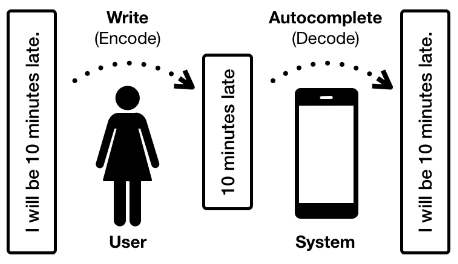
\includegraphics[width=.5\linewidth]{figs/autocomplete_game.png}
    \caption{schematic overview of the communication game. Figure from \protect\citeA{autocomplete}.}
    \label{fig:autocomplete}
\end{figure}

The same autocomplete communication game is considered as in \citeA{autocomplete}. In this game, a human (called user) encodes a sentence into keywords. 
These keywords are then decoded by a machine (called system) to retrieve the full, initial sentence. 
A schematic overview is given in figure \ref{fig:autocomplete}. 
The communication game is succesfull if the retrieved sentence is the same as the initial sentence. 

More formally, a target sentence $x=(x_1, \dots, x_m)$ is communicated by a user through the keywords $z=(z_1, \dots, z_n)$. 
Note that $z$ is a subsequence of $x$. 
The system then tries to retrieve the target sentence by decoding the keywords. 
The target sentence is described by the keywords using encoding strategy $q_{\alpha}(z | x)$ and the system decodes the keywords by using decoding strategy $p_{\beta}(x|z)$. 

For a model to be efficient, the number of keywords needs to be as low as possible. 
In addition, for a model to be accurate, the probability of reconstructing $x$ from $z$ needs to be as high as possible. 
Therefore, a cost and a loss, respectively, can be defined:
\begin{equation}
    \label{eq:cost}
    \text{cost}(x,\alpha) = \mathbb{E}_{q_{\alpha}(z|x)} [\text{length}(z)]
\end{equation}
\begin{equation}
    \label{eq:loss}
    \text{loss}(x,\alpha,\beta) = \mathbb{E}_{q_{\alpha}(z|x)} [-\log p_{\beta}(x|z)]
\end{equation}

\subsection{Segmentation model}
\label{sec:segmentation}
% Why does a segmentation model work?

\paragraph{General idea.}
If there is a rod of length $n$ and we can cut this rod at every marker, how can we best find the maximal total value of the resulting pieces?
This is called the rod cutting problem.
The segmentation model gives a solution to the rot cutting problem. 
The segmentation model takes the scores of all pieces of the rod, called segments. 
Those segments can be of length 1 or 2 or even $n$. 
With these scores, the model determines what the best possible segmentation is. 
To find the best segmentation and the probability of a segmentation, the model makes use of dynamic programming algorithms such as the Viterbi algorithm \cite{Viterbi} and the forward algorithm.
The segmentation model is essentially a simpler version of a hidden semi-Markov model \cite{hsmms}. 


\paragraph{Segmentation model for text.}
So how does the segmentation model work for text? 
If we have a sentence, e.g. \textit{'I will be late'}, we can use fencepost indexing and represent the fenceposts as nodes in a directed acyclic graph (DAG). 
This can be compared with the rod from before.
We can then draw edges between those nodes that represent segments. 
Those segments can be seen as (groups of) words. 
In figure \ref{fig:dag}, a DAG can be seen in which all the possible segments are showed. 
In the case of the autocomplete communication model described before, a segment is either kept or not.
Therefore, we can have one edge representing 'keep' and one representing 'do not keep', resulting in figure \ref{fig:dag2}.
If the pink edges are taken as 'do not keep' and the blue ones as 'keep', two possible segmentations can be seen in figure \ref{fig:segmentation} and \ref{fig:segmentation2}. 
Both segmentations result in the keywords \textit{'will be late'}. 

\begin{figure}
    \centering
    \begin{subfigure}[b]{0.45\textwidth}
        \centering
        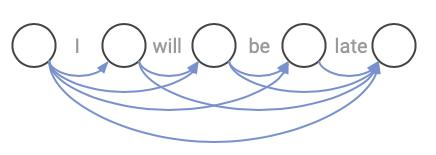
\includegraphics[width=\textwidth]{figs/segmentation1.jpeg}
        \caption{Possible segments in a DAG}
        \label{fig:dag}
    \end{subfigure}
    \hfill
    \begin{subfigure}[b]{0.45\textwidth}
        \centering
        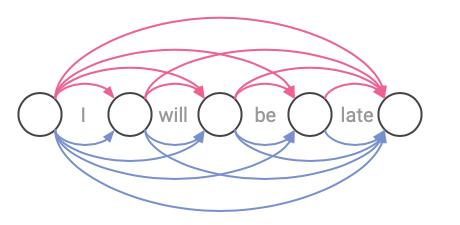
\includegraphics[width=\textwidth]{figs/segmentation2.jpeg}
        \caption{Possible segments in a DAG when each segment can either be true or false}
        \label{fig:dag2}
    \end{subfigure}
    \hfill
    \begin{subfigure}[b]{0.45\textwidth}
        \centering
        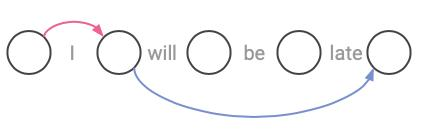
\includegraphics[width=\textwidth]{figs/segmentation3.jpeg}
        \caption{A possible segmentation}
        \label{fig:segmentation}
    \end{subfigure}
    \hfill
    \begin{subfigure}[b]{0.45\textwidth}
        \centering
        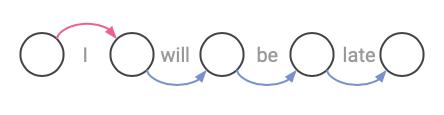
\includegraphics[width=\textwidth]{figs/segmentation4.jpeg}
        \caption{Another possible segmentation}
        \label{fig:segmentation2}
    \end{subfigure}
    \caption{Segmentation model}
    \label{fig:segmentation_model}
\end{figure}


\subsection{Structured latent variables}
A latent variable is an unobservable variable.
For these variables, there are no labels available. 
Therefore, it is not possible to use supervised learning on them. 
In the case of this model, we try to recover the full sentence by inferring what is a good mask.
The mask determines what words are good keywords and thus is a latent variable. 
In addition, the segmentation model makes this a structured variable. 

% Previous research on segmentations predicted a segmentation as output, rather than as a latent variable \cite{hsmms,conditionalRandomFields,kong2016segmentalrecurrentneuralnetworks}. 

\section{Current research}
% Gap
% Research question: To what extend can a segmentation model help by selecting keywords for an auto-complete communication game?
% TODO: check references - are they relevant?
% into account for what?

Previous research did not take structure into account \cite{autocomplete, Bar-YossefZiv2011Cqa, SvyatkovskiyAlexey2019PACC}.
Since language is structured, it makes sense to use a structured model as an autocomplete model. 
Furthermore, previous work has shown that the prediction of segmentations can lead to better results than models that do not explicitly represent segments \cite{conditionalRandomFields,kong2016segmentalrecurrentneuralnetworks}. 
Therefore, in this research, we look at how we can use a latent segmentation model to retrieve keywords from a sentence. 
The segmentation model will be implemented in the encoder of the encoder-decoder model in order to choose the best keywords from the sentence.